\documentclass{article}

\usepackage{graphicx}

\begin{document}
\newpage
   \vspace*{\stretch{1.0}}
   \begin{center}
      \Large\textbf{Earth 436B Thesis}\\
      \large\textit{John Lawson}
   \end{center}
   \vspace*{\stretch{2.0}}

\newpage
\section{Locations}   
-Grand Traverse Bay, Michigan (GTB)\\
-Au Train Bay, Michigan (ATB)\\
-Batchawana Bay, Ontario (BATB)\\
-Tahquamenon Bay, Michigan (TAHB)\\
\newpage
\section{Method}
-OSL dating used to determine age for sequences of late Holocene shoreline
deposits, (known as Strandplain sequences) at each site vs current day elevation.\\
-Not all strandplains were age dated due to coset, so a linear regression model of age vs horizontal distance along the strandplain sequence is used to estimate age values for strandplains that were not directly age dated.\\
-This is then used to create a graph of elevation vs time for each site\\
\newpage
\section[2]{Method}
-OSL dating used to determine age for sequences of Quaternary beach deposits (strandplain sequences) at each site vs current day elevation.\\
-This is then used to create a graph of elevation vs time for each site\\
\begin{figure}[h]
	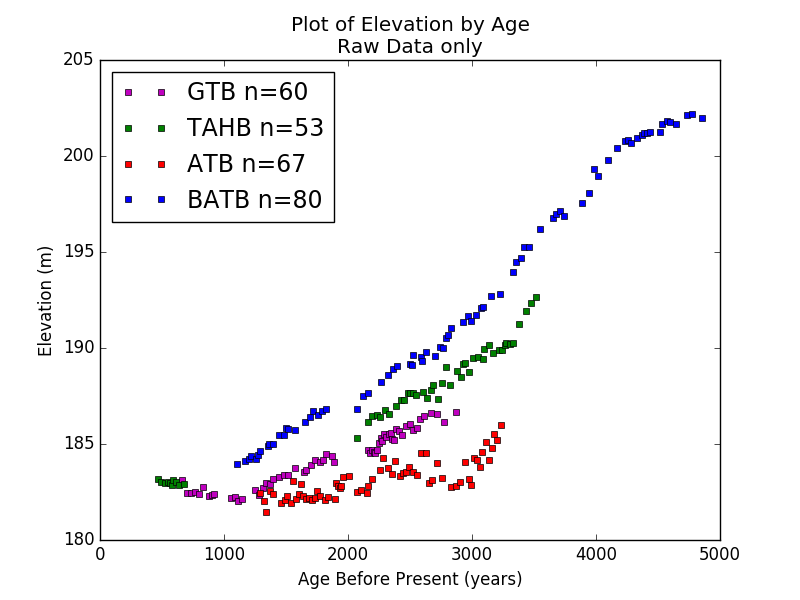
\includegraphics[width=\linewidth]{data/theDataRaw.png}
	\caption{Definitely not a boat.}
	\label{fig:rawData}
\end{figure}
\newpage
\section[2]{Method}
-Data not available continuously for each site, or at the same time for each site to compare gia, so values must be inferred using linear interpolation between known data points.\\
\begin{figure}[h]
	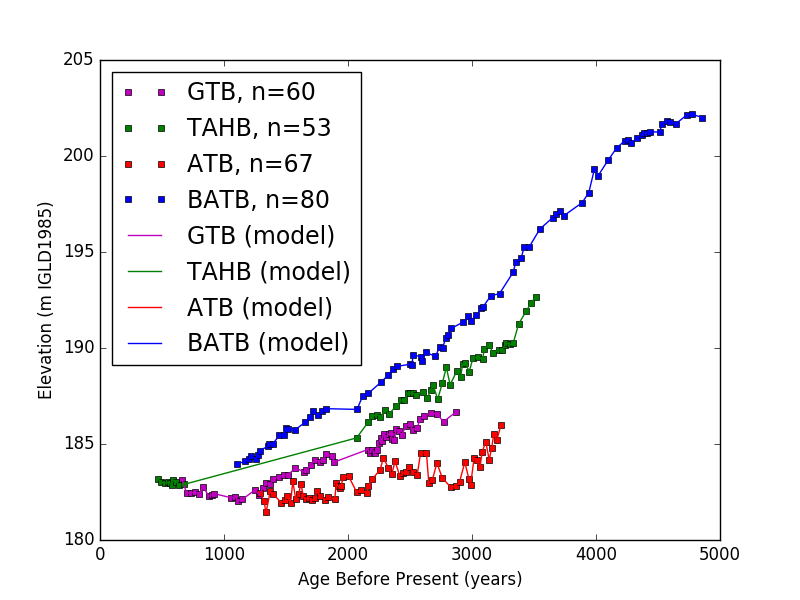
\includegraphics[width=\linewidth]{data/theData.png}
	\caption{Definitely not a boat.}
	\label{fig:dataWithModel}
\end{figure}
\newpage
\section[2]{Method}
-GIA is now plotted by subtracting between the measured values of one dataset and the modelled value of another.\\
-6 combinations of pairs of sites are created, each of which has a forward (A to B) and backward ()B to A) comparison.\\
\newpage
\begin{figure}[h]
	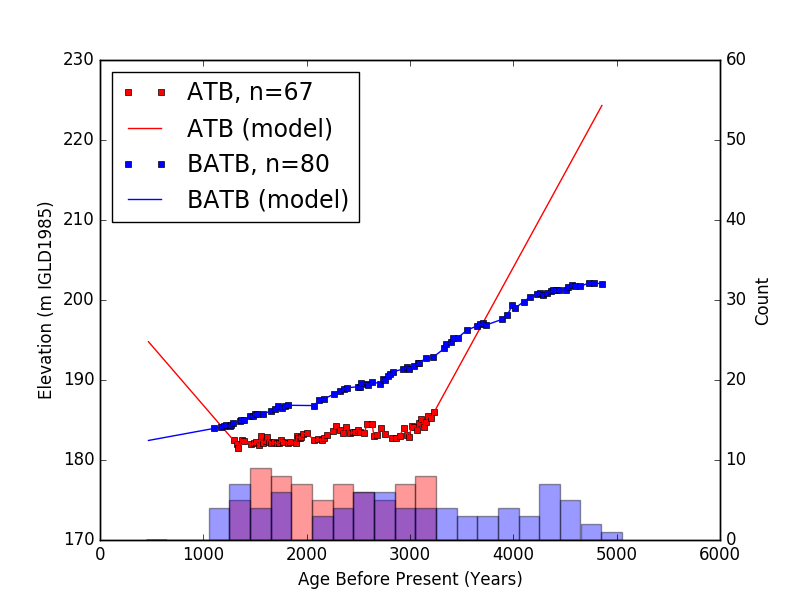
\includegraphics[width=\linewidth]{data/ATB-BATB_DataAndModel.png}
	\caption{Definitely not a boat.}
	\label{fig:data_ATBxBATB}
\end{figure}
\newpage

\begin{figure}[h]
	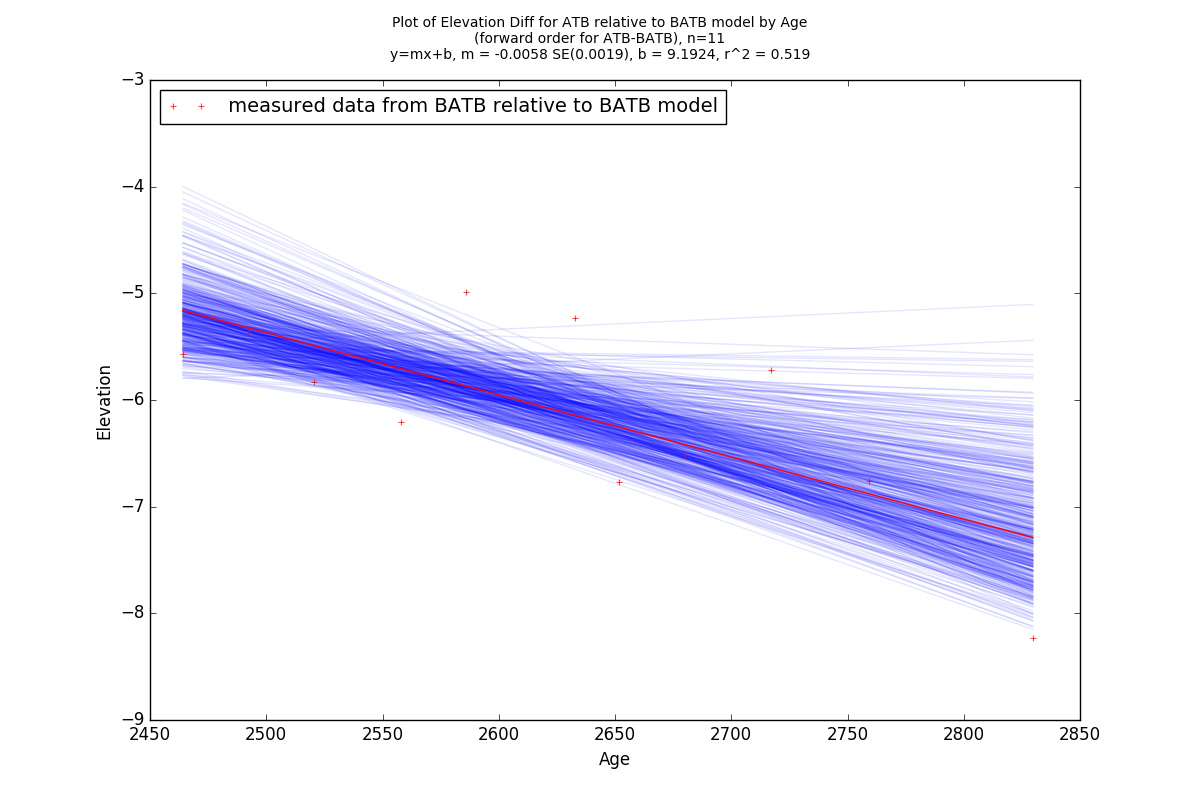
\includegraphics[width=\linewidth]{data/gias/theGIA_ATB_relative_to_BATB.png}
	\caption{Definitely not a boat.}
	\label{fig:gias_ATBxBATB}
\end{figure}
\newpage


\begin{figure}[h]
	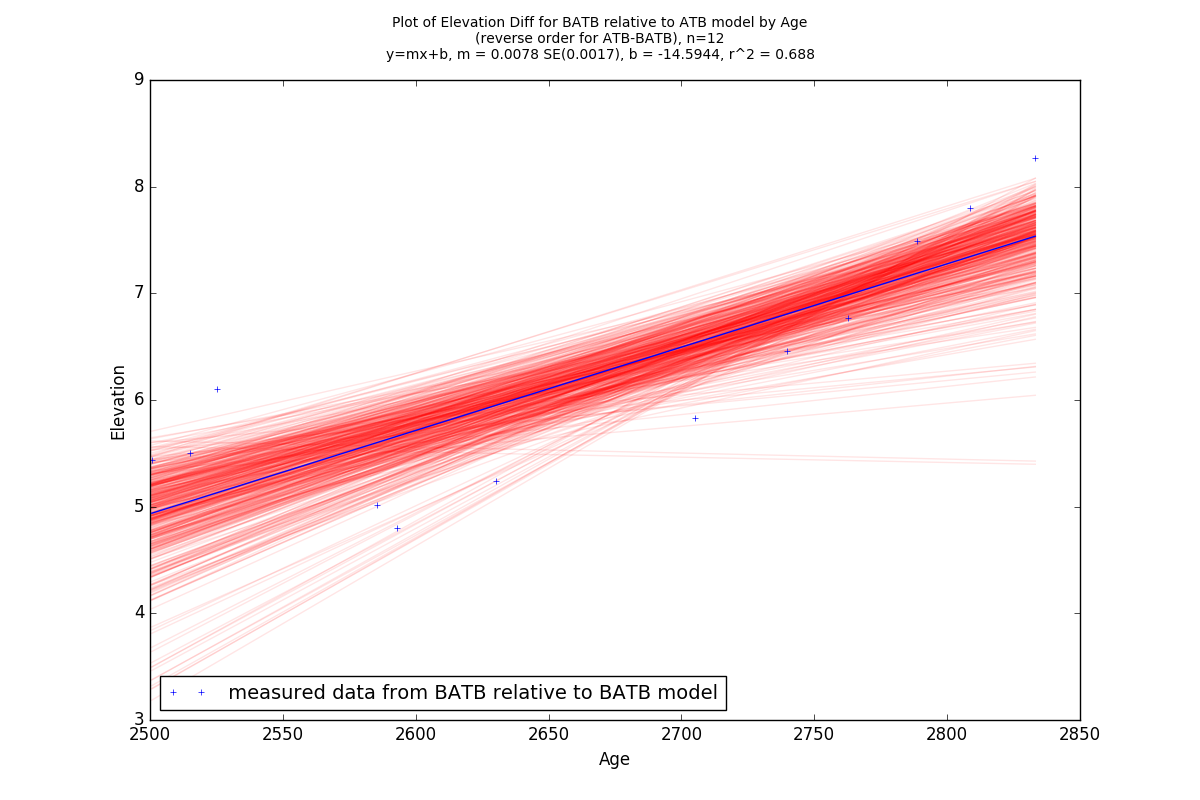
\includegraphics[width=\linewidth]{data/gias/theGIA_BATB_relative_to_ATB.png}
	\caption{Definitely not a boat.}
	\label{fig:gias_BATBxATB}
\end{figure}
\newpage
% this desperately needs to be done as a loop



\begin{figure}[h]
	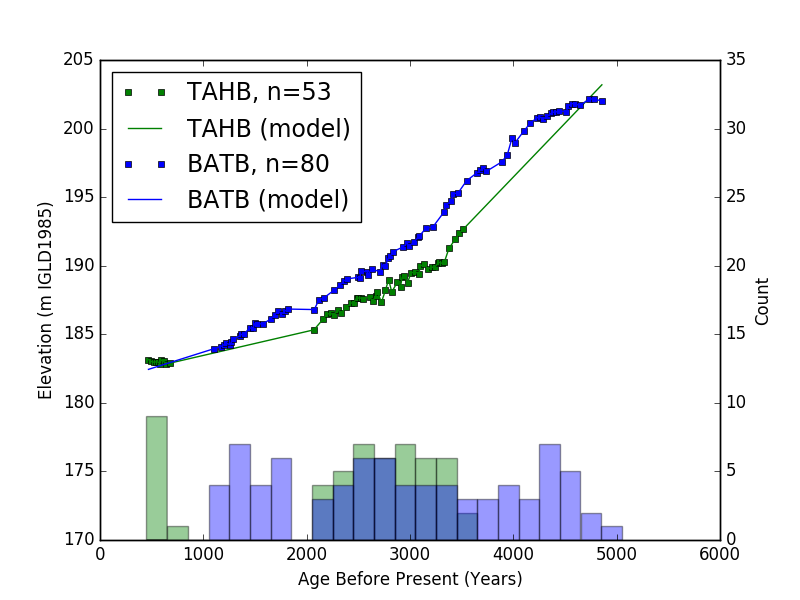
\includegraphics[width=\linewidth]{data/TAHB-BATB_DataAndModel.png}
	\caption{Definitely not a boat.}
	\label{fig:data_TAHBxBATB}
\end{figure}
\newpage

\begin{figure}[h]
	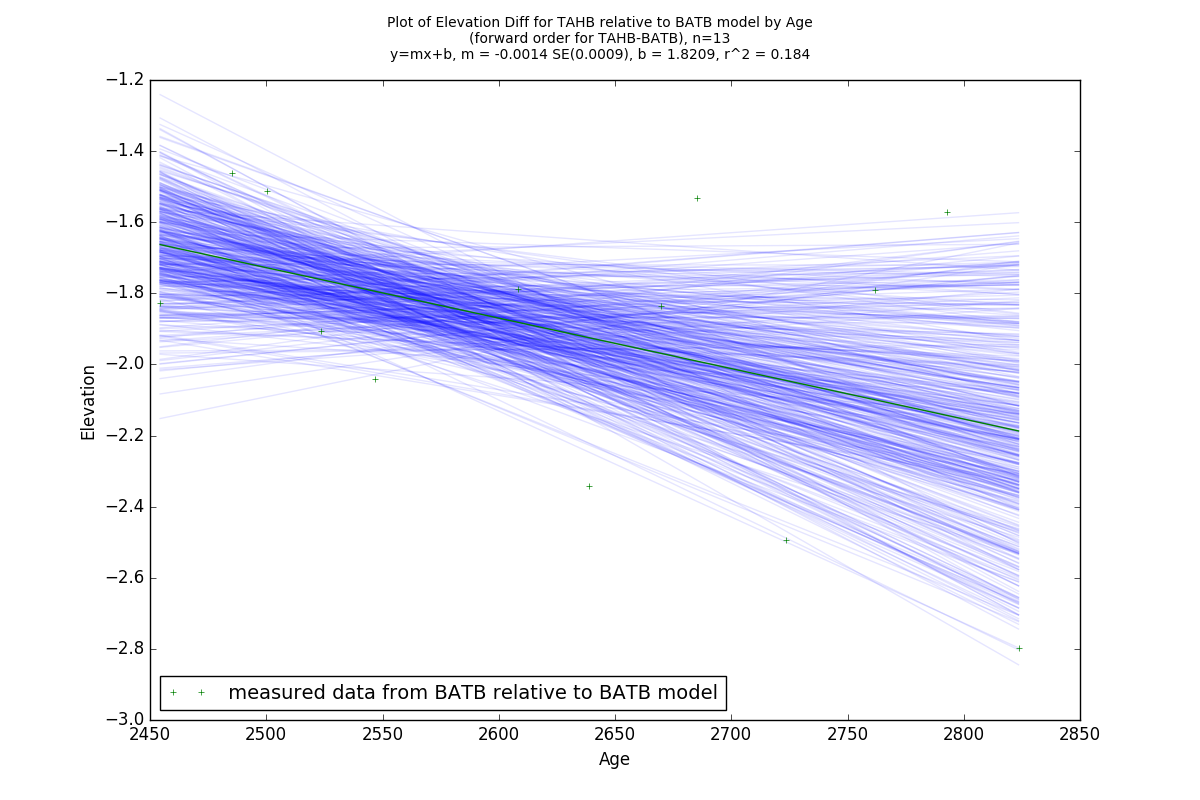
\includegraphics[width=\linewidth]{data/gias/theGIA_TAHB_relative_to_BATB.png}
	\caption{Definitely not a boat.}
	\label{fig:gias_TAHBxBATB}
\end{figure}
\newpage


\begin{figure}[h]
	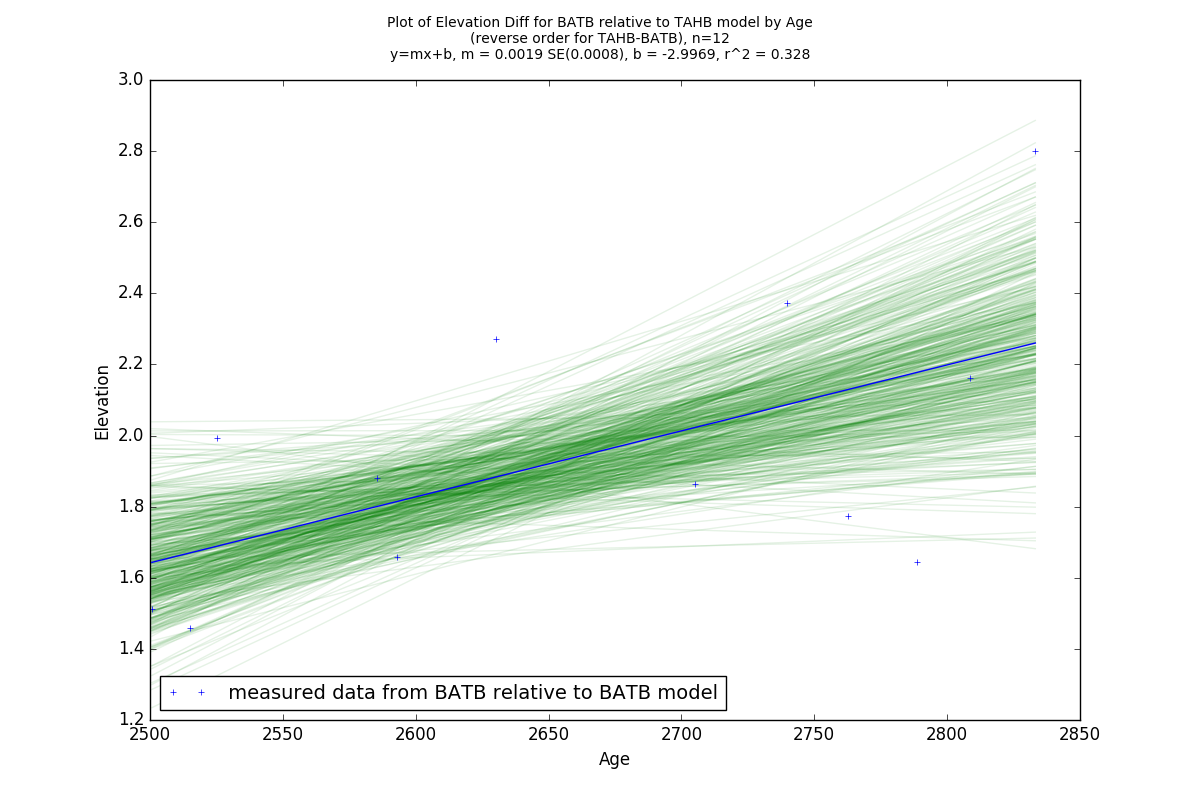
\includegraphics[width=\linewidth]{data/gias/theGIA_BATB_relative_to_TAHB.png}
	\caption{Definitely not a boat.}
	\label{fig:gias_BATBxTAHB}
\end{figure}
\newpage








\begin{figure}[h]
	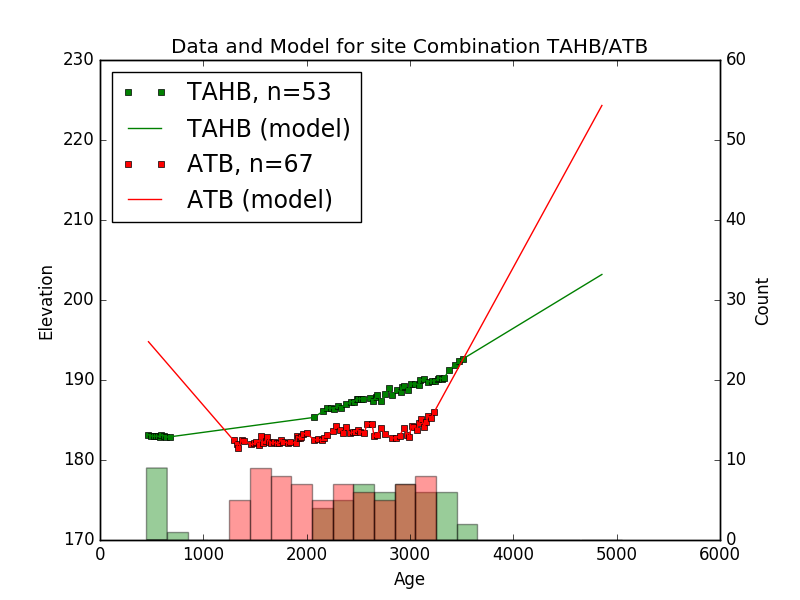
\includegraphics[width=\linewidth]{data/TAHB-ATB_DataAndModel.png}
	\caption{Definitely not a boat.}
	\label{fig:data_TAHBxBATB}
\end{figure}
\newpage

\begin{figure}[h]
	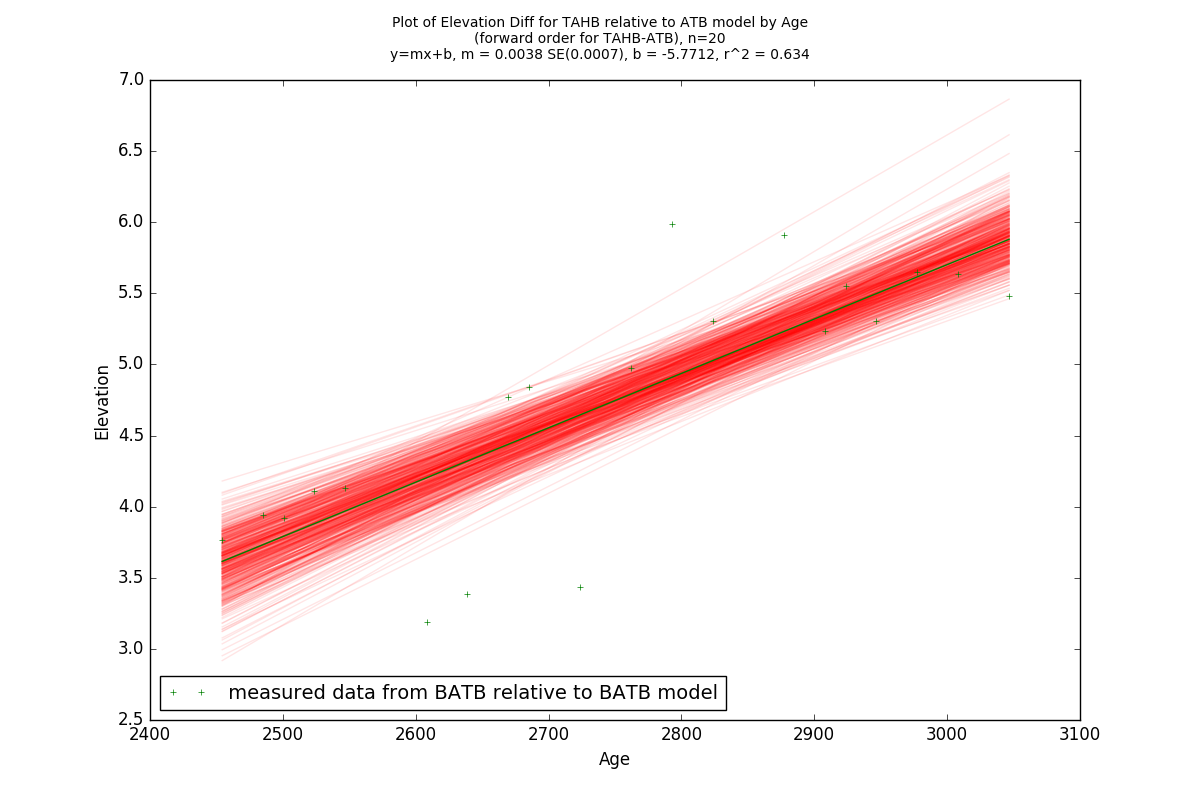
\includegraphics[width=\linewidth]{data/gias/theGIA_TAHB_relative_to_ATB.png}
	\caption{Definitely not a boat.}
	\label{fig:gias_TAHBxATB}
\end{figure}
\newpage


\begin{figure}[h]
	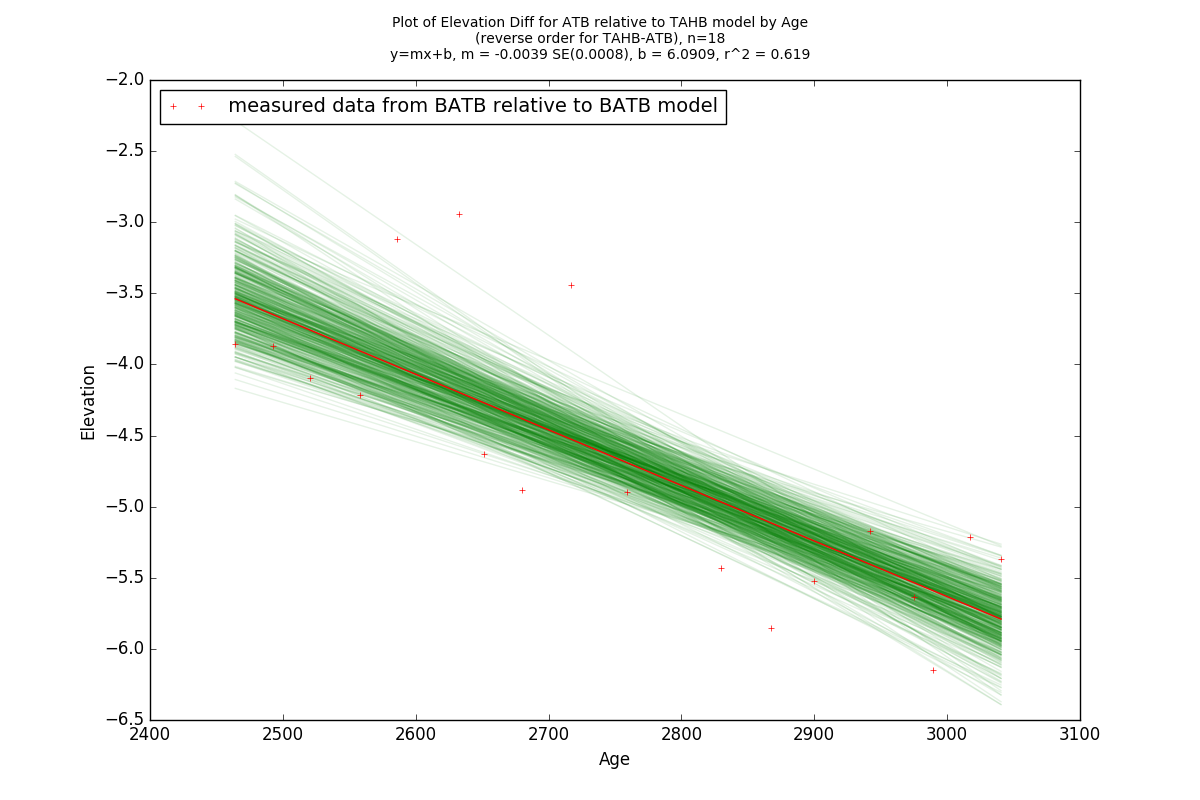
\includegraphics[width=\linewidth]{data/gias/theGIA_ATB_relative_to_TAHB.png}
	\caption{Definitely not a boat.}
	\label{fig:gias_ATBxTAHB}
\end{figure}
\newpage






\begin{figure}[h]
	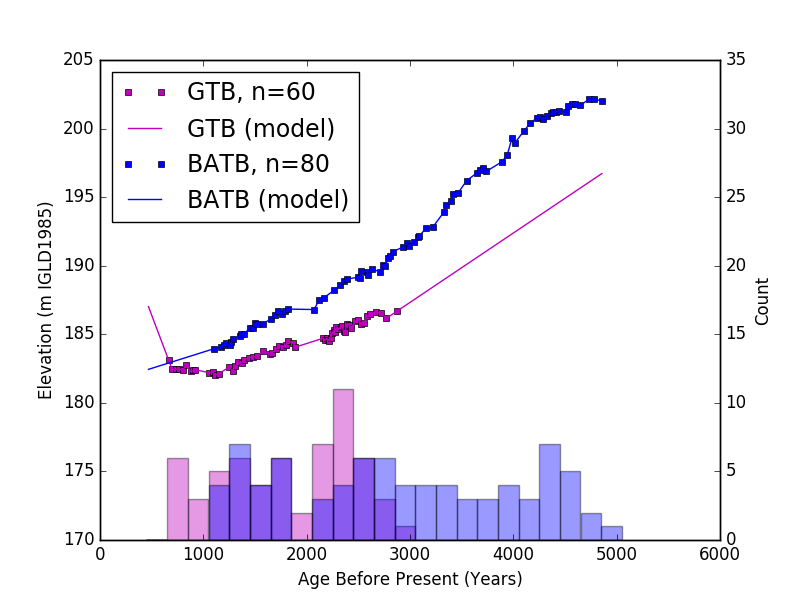
\includegraphics[width=\linewidth]{data/GTB-BATB_DataAndModel.png}
	\caption{Definitely not a boat.}
	\label{fig:data_GTBxBATB}
\end{figure}
\newpage

\begin{figure}[h]
	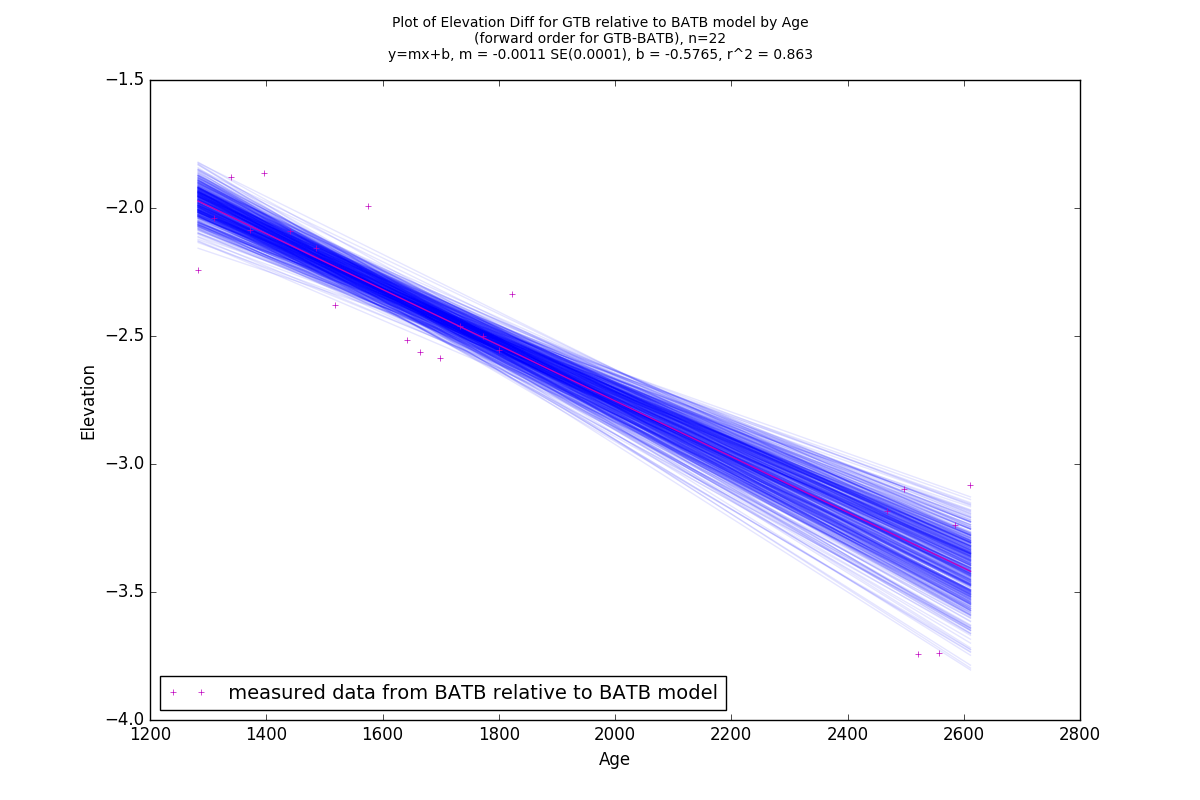
\includegraphics[width=\linewidth]{data/gias/theGIA_GTB_relative_to_BATB.png}
	\caption{Definitely not a boat.}
	\label{fig:gias_GTBxBATB}
\end{figure}
\newpage


\begin{figure}[h]
	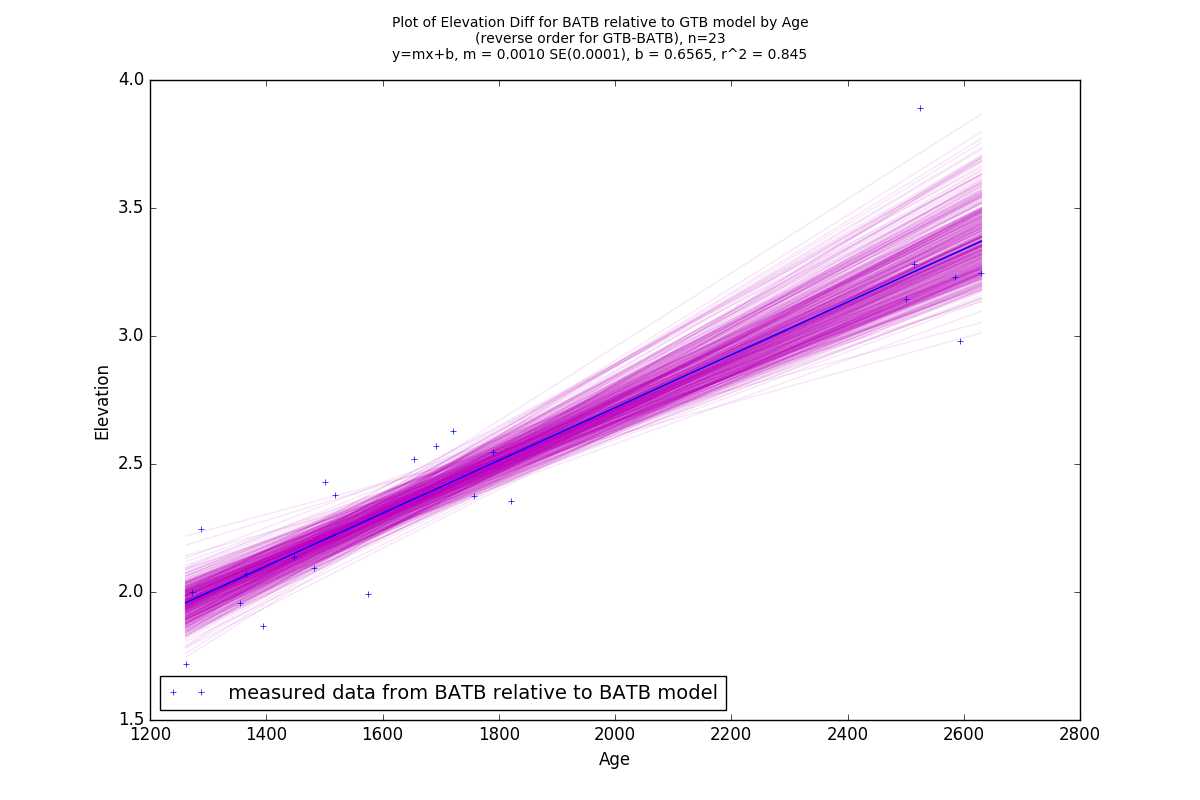
\includegraphics[width=\linewidth]{data/gias/theGIA_BATB_relative_to_GTB.png}
	\caption{Definitely not a boat.}
	\label{fig:gias_BATBxGTB}
\end{figure}
\newpage









\begin{figure}[h]
	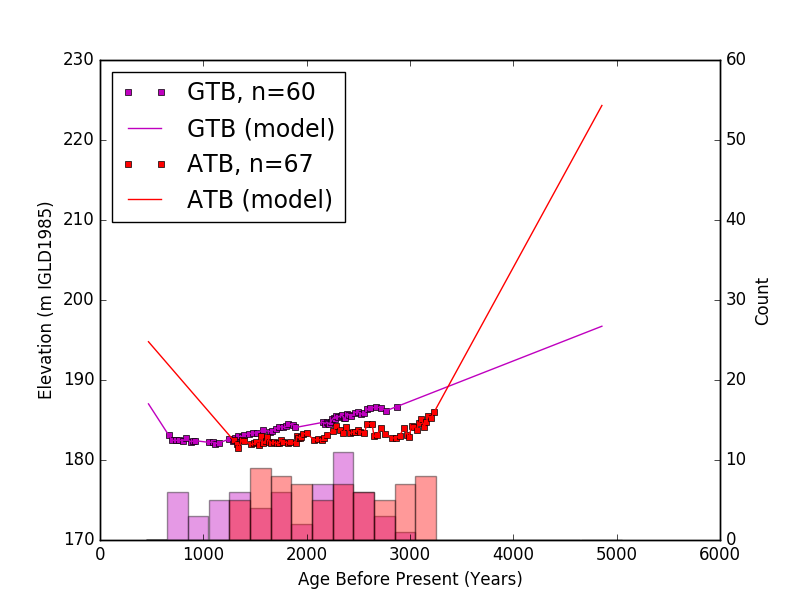
\includegraphics[width=\linewidth]{data/GTB-ATB_DataAndModel.png}
	\caption{Definitely not a boat.}
	\label{fig:data_GTBxATB}
\end{figure}
\newpage

\begin{figure}[h]
	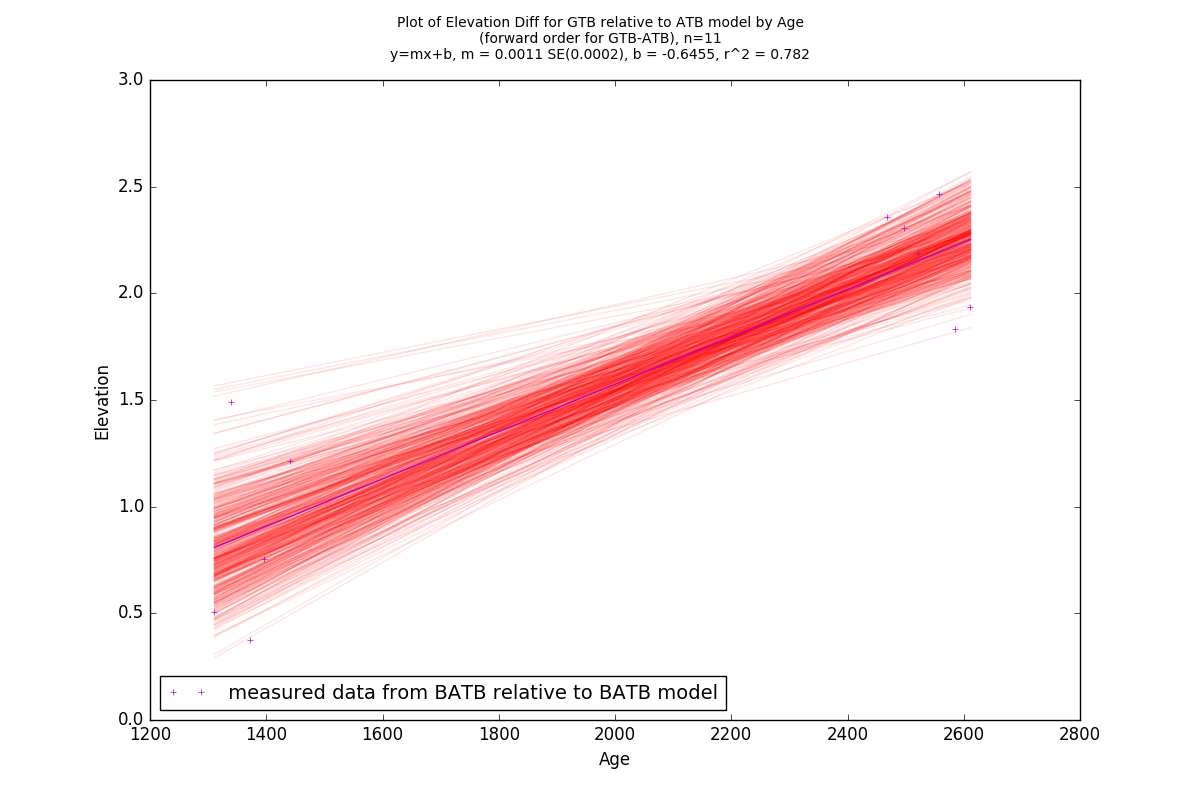
\includegraphics[width=\linewidth]{data/gias/theGIA_GTB_relative_to_ATB.png}
	\caption{Definitely not a boat.}
	\label{fig:gias_GTBxATB}
\end{figure}
\newpage


\begin{figure}[h]
	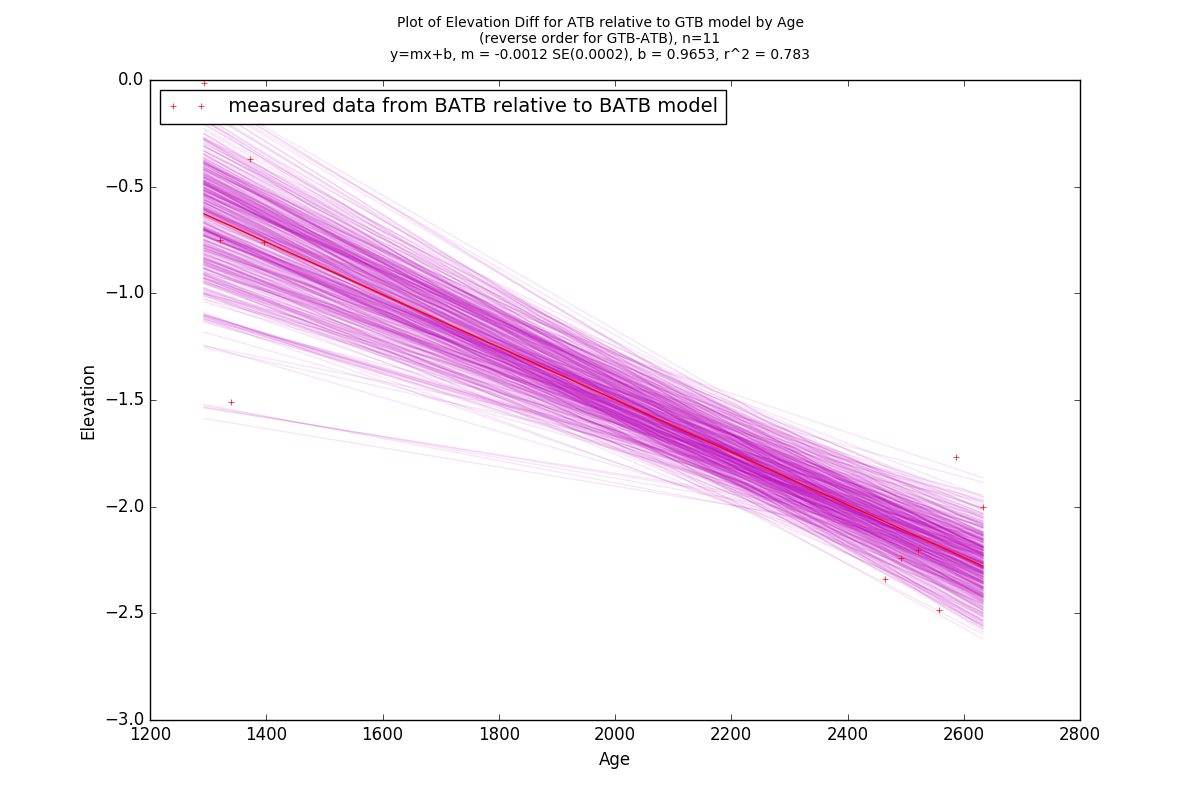
\includegraphics[width=\linewidth]{data/gias/theGIA_ATB_relative_to_GTB.png}
	\caption{Definitely not a boat.}
	\label{fig:gias_ATBxGTB}
\end{figure}
\newpage










\begin{figure}[h]
	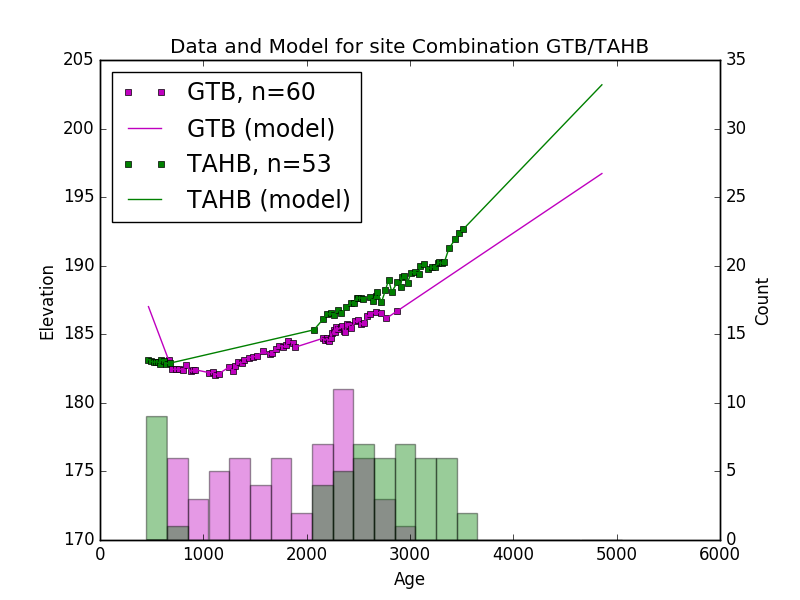
\includegraphics[width=\linewidth]{data/GTB-TAHB_DataAndModel.png}
	\caption{Definitely not a boat.}
	\label{fig:data_GTBxTAHB}
\end{figure}
\newpage

\begin{figure}[h]
	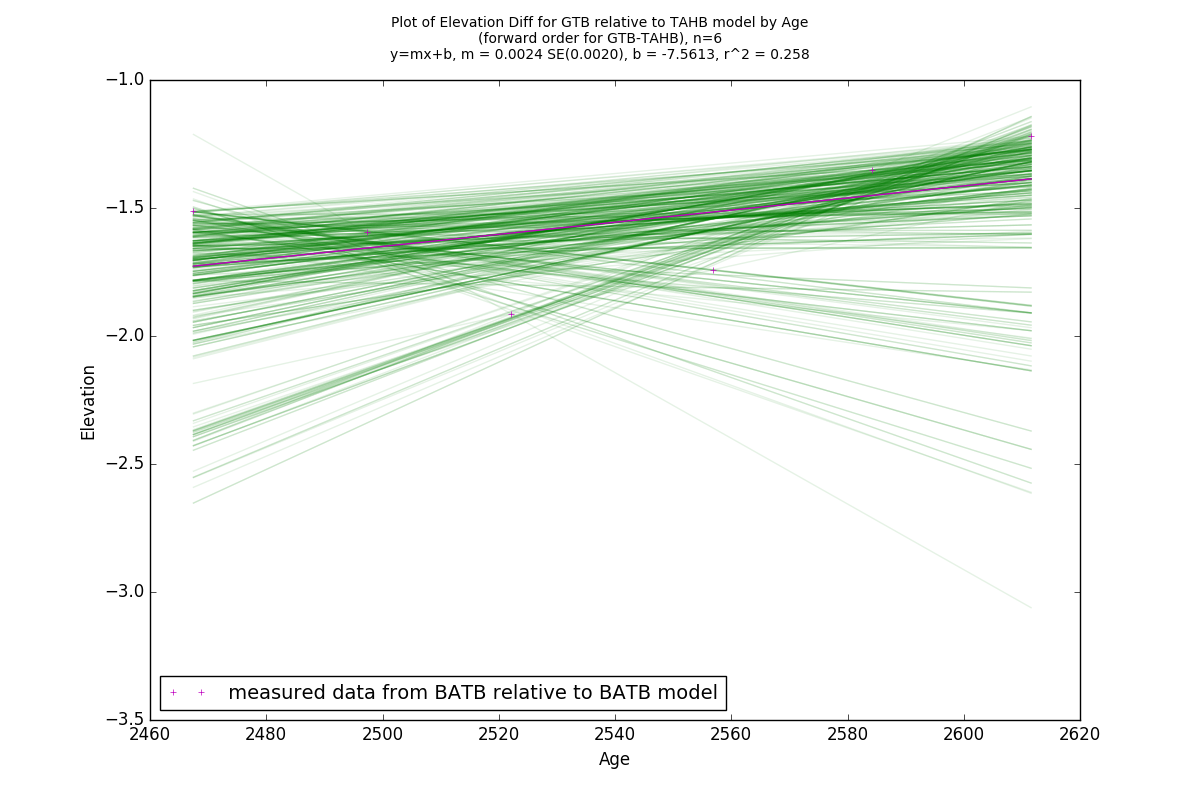
\includegraphics[width=\linewidth]{data/gias/theGIA_GTB_relative_to_TAHB.png}
	\caption{Definitely not a boat.}
	\label{fig:gias_GTBxTAHB}
\end{figure}
\newpage


\begin{figure}[h]
	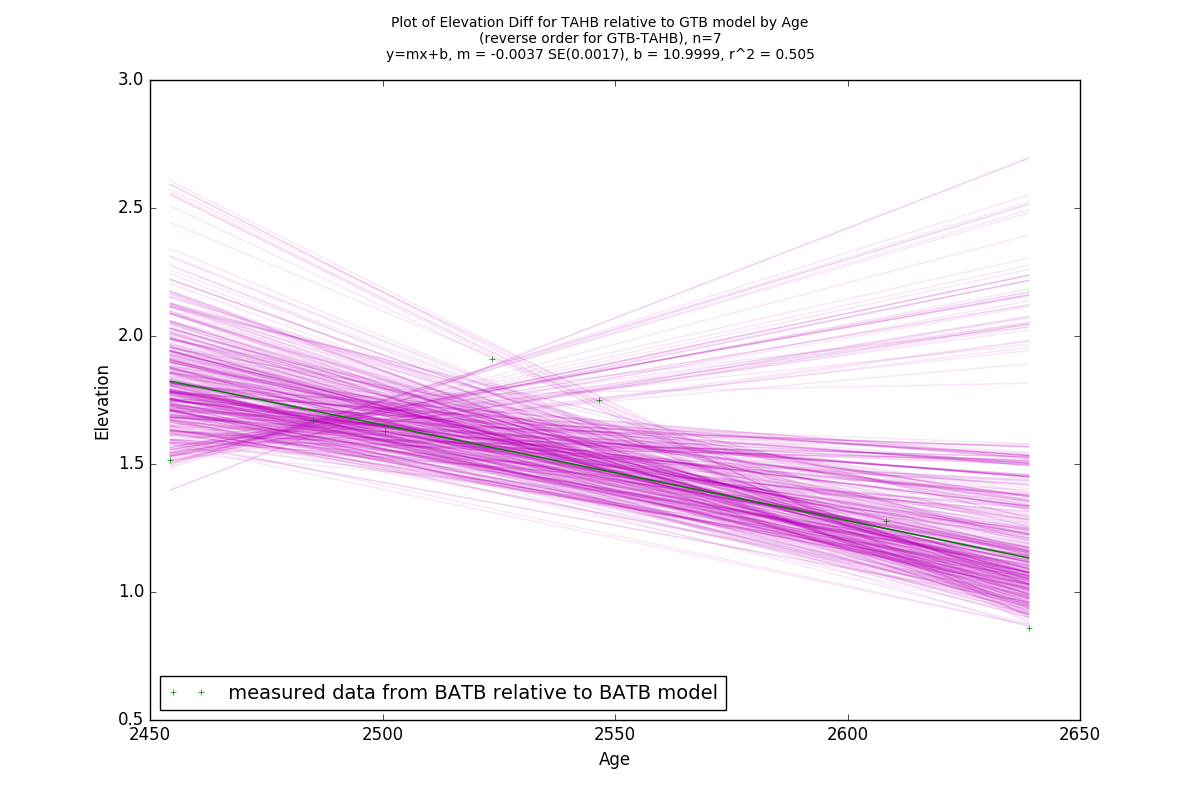
\includegraphics[width=\linewidth]{data/gias/theGIA_TAHB_relative_to_GTB.png}
	\caption{Definitely not a boat.}
	\label{fig:gias_TAHBxGTB}
\end{figure}
\newpage







\end{document}
